\documentclass{standalone}
\usepackage{tikz}
\usepackage{xcolor}

\begin{document}
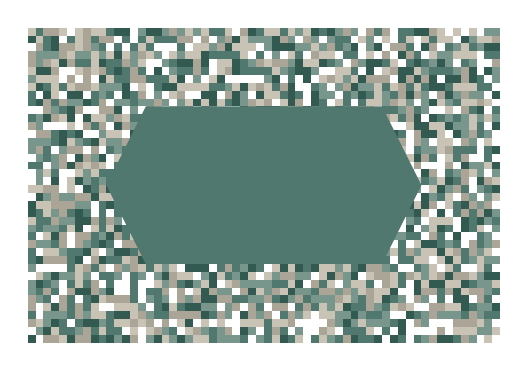
\begin{tikzpicture}[scale=0.1] % Ajusta la escala según sea necesario

% Definición de colores basados en la imagen (puedes ajustarlos)
\definecolor{color1}{RGB}{230, 225, 210} % Beige claro
\definecolor{color2}{RGB}{200, 195, 180} % Beige medio
\definecolor{color3}{RGB}{170, 165, 150} % Beige oscuro
\definecolor{color4}{RGB}{120, 150, 140} % Verde azulado claro
\definecolor{color5}{RGB}{80, 120, 110}  % Verde azulado medio
\definecolor{color6}{RGB}{50, 90, 80}   % Verde azulado oscuro

% Patrón de cuadrados y colores (ajusta según la imagen)
\foreach \x in {0,1,...,59} {
  \foreach \y in {0,1,...,39} {
    \pgfmathsetmacro{\randomColor}{random(1,6)}
    \ifcase\randomColor
      \fill[color1] (\x,\y) rectangle ++(1,1);
    \or
      \fill[color2] (\x,\y) rectangle ++(1,1);
    \or
      \fill[color3] (\x,\y) rectangle ++(1,1);
    \or
      \fill[color4] (\x,\y) rectangle ++(1,1);
    \or
      \fill[color5] (\x,\y) rectangle ++(1,1);
    \or
      \fill[color6] (\x,\y) rectangle ++(1,1);
    \fi
  }
}

% Dibujo de la forma central (ajusta las coordenadas según la imagen)
\fill[color5] (15,10) -- (45,10) -- (50,20) -- (45,30) -- (15,30) -- (10,20) -- cycle;

\end{tikzpicture}
\end{document}